\def\SECTION{1.4 Perimeter \& Area}
\documentclass[aspectratio=169,14pt]{beamer}
\usepackage[T1]{fontenc}
\usepackage{mathpazo}
\usepackage{amsmath,amssymb}
\usepackage{tikz}
\usetikzlibrary{arrows.meta,calc,decorations.pathreplacing}
\definecolor{fblue}{HTML}{1F4E79}
\definecolor{fteal}{HTML}{0F7C7C}
\definecolor{fgold}{HTML}{C9962B}
\definecolor{fred}{HTML}{B3261E}
\definecolor{fink}{HTML}{16233B}
\definecolor{fsoft}{HTML}{EEF3F8}
\definecolor{fgoldsoft}{HTML}{FBF1DC}
\setbeamertemplate{navigation symbols}{}
\setbeamercolor{normal text}{fg=fink}
\setbeamercolor{frametitle}{fg=fblue}
\setbeamerfont{frametitle}{series=\bfseries,size=\Large}
\setbeamercolor{structure}{fg=fteal}
\setbeamertemplate{itemize item}{\color{fteal}$\blacktriangleright$}
\setbeamertemplate{frametitle}{\vspace{6pt}\insertframetitle\par\vspace{-2pt}{\color{fgold}\rule{2.2cm}{2pt}}}
\setbeamertemplate{footline}{\hspace{0.6cm}{\color{fblue}\scriptsize\bfseries Prof.\ Fang \textcolor{fteal}{Math}}\hfill{\scriptsize\color{gray}\SECTION\quad\insertframenumber}\hspace{0.6cm}\vspace{6pt}}
\newcommand{\key}[1]{{\color{fteal}\textbf{#1}}}
\newcommand{\ans}[1]{\colorbox{fgoldsoft}{\color{fink}\ensuremath{#1}}}
\newcommand{\warn}[1]{\begin{beamercolorbox}[sep=8pt,rounded=true]{warnbox}{\color{fred}\textbf{Watch out!}}\enskip #1\end{beamercolorbox}}
\setbeamercolor{warnbox}{bg=fred!8,fg=fink}
\setbeamercolor{turnbox}{bg=fgoldsoft,fg=fink}
\setbeamercolor{defbox}{bg=fsoft,fg=fink}
\newcommand{\defn}[1]{\begin{beamercolorbox}[sep=8pt,rounded=true]{defbox}#1\end{beamercolorbox}}
\newenvironment{yourturn}{\begin{beamercolorbox}[sep=10pt,rounded=true]{turnbox}{\color{fgold}\Large\bfseries Your turn!}\quad{\small Pause the video and try it.}\par\medskip}{\end{beamercolorbox}}
\newcommand{\titleframe}[3]{%
\begin{frame}[plain]
\begin{tikzpicture}[remember picture,overlay]
\fill[fblue] (current page.north west) rectangle ([yshift=-0.9cm]current page.north east);
\node[anchor=west,text=white,font=\bfseries] at ([xshift=0.6cm,yshift=-0.45cm]current page.north west) {Prof.\ Fang \textcolor{fgold}{Math}};
\node[anchor=east,text=white,font=\small] at ([xshift=-0.6cm,yshift=-0.45cm]current page.north east) {Geometry $\cdot$ Chapter 1};
\end{tikzpicture}
\vfill
{\color{fteal}\large\bfseries #1}\par\medskip
{\color{fblue}\fontsize{30}{34}\selectfont\bfseries #2}\par\medskip
{\color{fgold}\rule{3cm}{3pt}}\par\bigskip
{\large #3}
\vfill
{\small\color{gray} fangmath.com $\cdot$ YouTube @3SMath}
\end{frame}}
\newcommand{\closeframe}[1]{%
\begin{frame}{Remember}
#1
\vfill
\begin{center}{\color{fblue}\large\bfseries Now practice at your level:}\par\smallskip
{\Large\color{fteal}\bfseries fangmath.com} \enskip{\color{gray}$\to$ Geometry $\to$ Chapter 1}\end{center}
\end{frame}}

\usepackage{pgfplots}\pgfplotsset{compat=1.17}
\newcommand{\grid}[4]{\draw[step=1,gray!25] (#1,#2) grid (#3,#4);\draw[-{Stealth},gray] (#1,0)--(#3+0.3,0) node[right]{\small$x$};\draw[-{Stealth},gray] (0,#2)--(0,#4+0.3) node[above]{\small$y$};}
\usetikzlibrary{angles,quotes}
\begin{document}
\titleframe{Lesson 1.4}{Perimeter \& Area in the Coordinate Plane}{Count the sides, then use the formulas you know}

\begin{frame}{Side lengths from coordinates}
\begin{columns}[c]
\begin{column}{0.5\textwidth}\centering
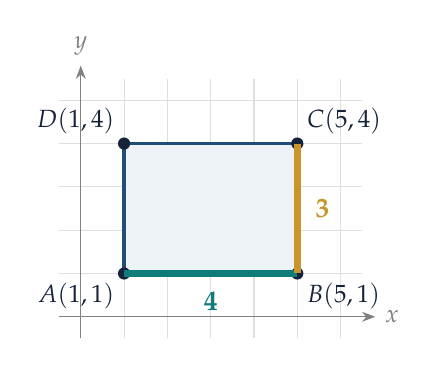
\begin{tikzpicture}[scale=0.55]
\grid{-0.5}{-0.5}{6.5}{5.5}
\draw[very thick,fblue,fill=fsoft] (1,1)--(5,1)--(5,4)--(1,4)--cycle;
\fill[fink] (1,1) circle(4pt) node[below left]{\small$A(1,1)$} (5,1) circle(4pt) node[below right]{\small$B(5,1)$} (5,4) circle(4pt) node[above right]{\small$C(5,4)$} (1,4) circle(4pt) node[above left]{\small$D(1,4)$};
\onslide<2->{\draw[fteal,line width=2.5pt] (1,1)--(5,1) node[midway,below=2pt]{\bfseries 4};}
\onslide<3->{\draw[fgold,line width=2.5pt] (5,1)--(5,4) node[midway,right=2pt]{\bfseries 3};}
\end{tikzpicture}
\end{column}
\begin{column}{0.48\textwidth}
Rectangle $ABCD$\par\medskip
\onslide<2->{$AB = 5 - 1 = 4$}\par\smallskip
\onslide<3->{$BC = 4 - 1 = 3$}\par\bigskip
\onslide<4->{\defn{Same $y$: subtract the $x$'s.\\ Same $x$: subtract the $y$'s.}}
\end{column}
\end{columns}
\end{frame}

\begin{frame}{Perimeter and area}
\begin{columns}[c]
\begin{column}{0.4\textwidth}\centering
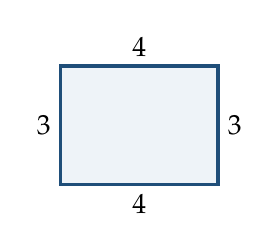
\begin{tikzpicture}[scale=0.5]
\draw[very thick,fblue,fill=fsoft] (0,0) rectangle (4,3);
\node[below] at (2,0){$4$}; \node[right] at (4,1.5){$3$}; \node[above] at (2,3){$4$}; \node[left] at (0,1.5){$3$};
\end{tikzpicture}
\end{column}
\begin{column}{0.58\textwidth}
\onslide<1->{\key{Perimeter} = add all the sides\par $P = 4 + 3 + 4 + 3 = \ans{14}$}\par\bigskip
\onslide<2->{\key{Area} = base $\times$ height\par $A = 4 \cdot 3 = \ans{12}$}\par\bigskip
\onslide<3->{{\small\color{gray} Perimeter is a length: \textbf{units}. Area counts squares: \textbf{square units}.}}
\end{column}
\end{columns}
\end{frame}

\begin{frame}{Area of a triangle}
\begin{columns}[c]
\begin{column}{0.5\textwidth}\centering
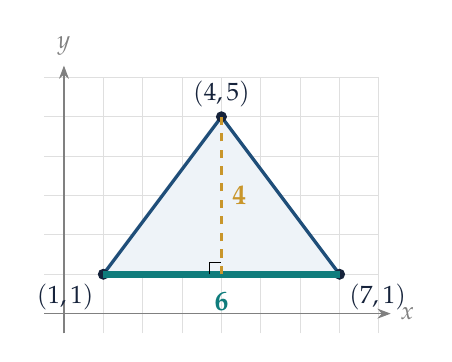
\begin{tikzpicture}[scale=0.5]
\grid{-0.5}{-0.5}{8}{6}
\draw[very thick,fblue,fill=fsoft] (1,1)--(7,1)--(4,5)--cycle;
\fill[fink] (1,1) circle(4pt) node[below left]{\small$(1,1)$} (7,1) circle(4pt) node[below right]{\small$(7,1)$} (4,5) circle(4pt) node[above]{\small$(4,5)$};
\onslide<2->{\draw[fteal,line width=2.5pt] (1,1)--(7,1) node[midway,below=2pt]{\bfseries 6};}
\onslide<3->{\draw[fgold,very thick,dashed] (4,1)--(4,5) node[midway,right]{\bfseries 4}; \draw (3.7,1)--(3.7,1.3)--(4,1.3);}
\end{tikzpicture}
\end{column}
\begin{column}{0.48\textwidth}
\onslide<2->{base $= 7 - 1 = 6$}\par\smallskip
\onslide<3->{height $= 5 - 1 = 4$\par{\small\color{gray} straight up from the base}}\par\bigskip
\onslide<4->{$A = \tfrac12 \cdot b \cdot h = \tfrac12 \cdot 6 \cdot 4 = \ans{12}$}
\end{column}
\end{columns}
\end{frame}

\begin{frame}{A slanted side? Use Pythagoras}
\begin{columns}[c]
\begin{column}{0.5\textwidth}\centering
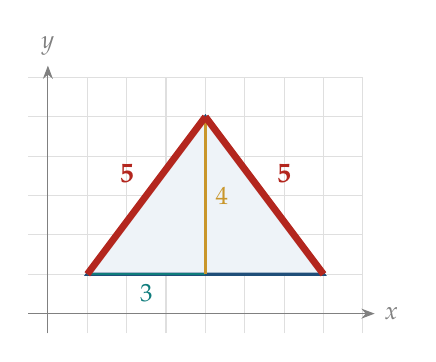
\begin{tikzpicture}[scale=0.5]
\grid{-0.5}{-0.5}{8}{6}
\draw[very thick,fblue,fill=fsoft] (1,1)--(7,1)--(4,5)--cycle;
\onslide<2->{\draw[fteal,thick] (1,1)--(4,1) node[midway,below]{\small 3}; \draw[fgold,thick] (4,1)--(4,5) node[midway,right]{\small 4}; \draw[fred,line width=2.5pt] (1,1)--(4,5) node[midway,above left]{\bfseries 5};}
\onslide<3->{\draw[fred,line width=2.5pt] (7,1)--(4,5) node[midway,above right]{\bfseries 5};}
\end{tikzpicture}
\end{column}
\begin{column}{0.48\textwidth}
\onslide<2->{Across 3, up 4:\par $\sqrt{3^2 + 4^2} = \sqrt{25} = 5$}\par\bigskip
\onslide<3->{The other side is also 5.\par\medskip $P = 6 + 5 + 5 = \ans{16}$}
\end{column}
\end{columns}
\end{frame}

\begin{frame}{Watch out}
\vfill
\warn{For a \textbf{slanted} side you can't just count squares. Use the Distance Formula --- or draw the right triangle and use Pythagoras.}
\vfill
\end{frame}

\begin{frame}{}
\begin{columns}[c]
\begin{column}{0.58\textwidth}
\begin{yourturn}
Triangle $P(0,0)$, $Q(6,0)$, $R(0,8)$.\par\smallskip Find its perimeter and area.
\end{yourturn}
\onslide<2->{\medskip
$PQ = 6,\ PR = 8$\par
$QR = \sqrt{6^2 + 8^2} = \sqrt{100} = 10$\par\smallskip
$P = 6 + 8 + 10 = \ans{24}$\par\smallskip
$A = \tfrac12 \cdot 6 \cdot 8 = \ans{24}$}
\end{column}
\begin{column}{0.4\textwidth}\centering
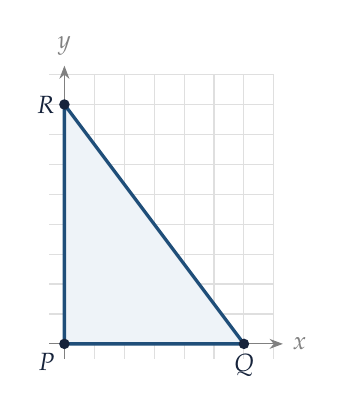
\begin{tikzpicture}[scale=0.38]
\grid{-0.5}{-0.5}{7}{9}
\draw[very thick,fblue,fill=fsoft] (0,0)--(6,0)--(0,8)--cycle;
\fill[fink] (0,0) circle(5pt) node[below left]{\small$P$} (6,0) circle(5pt) node[below]{\small$Q$} (0,8) circle(5pt) node[left]{\small$R$};
\end{tikzpicture}
\end{column}
\end{columns}
\end{frame}

\closeframe{\begin{itemize}\setlength\itemsep{10pt}
\item Same $y$: subtract the $x$'s. \ Same $x$: subtract the $y$'s.
\item \key{Perimeter}: add the sides. \ \key{Area}: rectangle $b \cdot h$, triangle $\tfrac12 b h$.
\item Slanted side: Pythagoras or the Distance Formula.
\end{itemize}}
\end{document}
